\chapter{Darstellung der Ergebnisse}
\label{c:Ergebnisse}

\section{Daten zum Flugversuch der DO-128}

\subsection{Auftriebsbeiwert $C_A$ über Widerstandsbeiwert $C_{W}$}

\begin{figure}[H]
	\centering	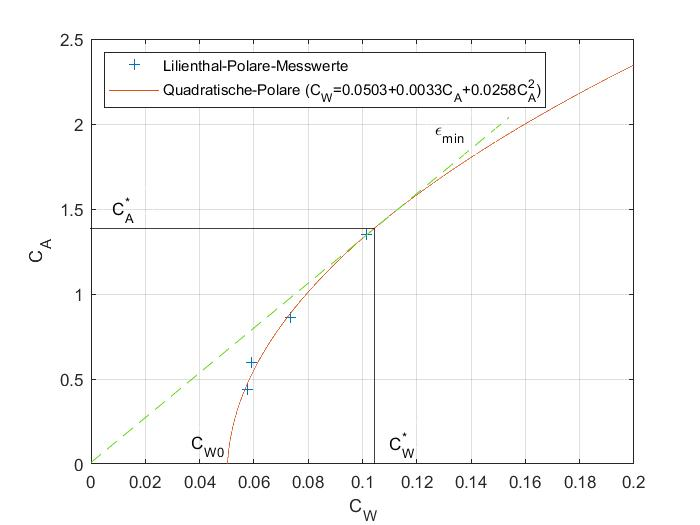
\includegraphics[width=0.7\textwidth]{./Bilder/CA_CW_DO128_NEU.jpg}
	\caption{$C_{A}$ über $C_{W}$ der DO-128}
	\label{fig:CA_CW_DO128}
\end{figure}

\subsection{Widerstand $W$ über Fluggeschwindigkeit $V$}
\label{ss:W_V}

\begin{figure}[H]
	\centering	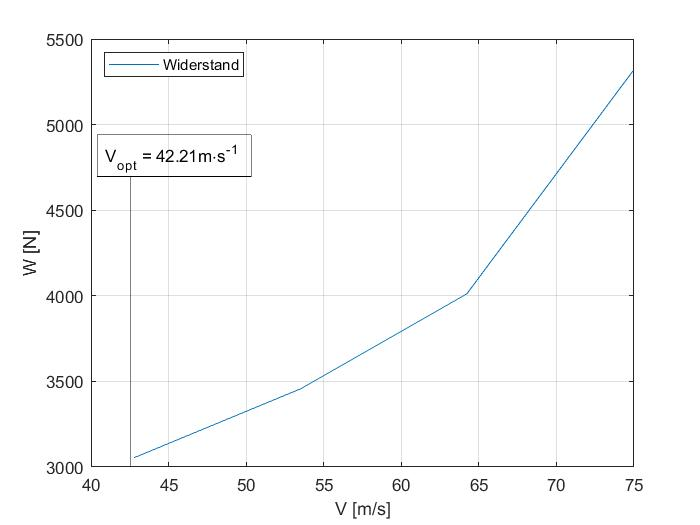
\includegraphics[width=0.7\textwidth]{./Bilder/W_V_DO128_NEU.jpg}
	\caption{$W$ über $V$ der DO-128}
	\label{fig:W_V_DO128}
\end{figure}

Die optimale Fluggeschwindigkeit $V_{opt}$ wurde, wie auch der minimale Widerstand $W_{min}$ (Im Graph nicht zu sehen), mittels der beiden Gleichungen \ref{eq:V_opt} und \ref{eq:W_min} definiert. Dazu wurde die Masse bzw. die Gewichtskraft $G$ des Flugzeugs, sowie die Dichte $\rho$ über die vier Flugabschnitte zu \SI{4142}{\ \kilogram} bzw. \SI{40633}{\ \newton} und 1,13 \SI{}{\kilogram\ \meter^{-3}} gemittelt.

\section{Daten zum Flugversuch der DO-28}

\subsection{Anstellwinkel $\alpha$ über Trimmwinkel $\eta$}

\begin{figure}[H]
	\centering	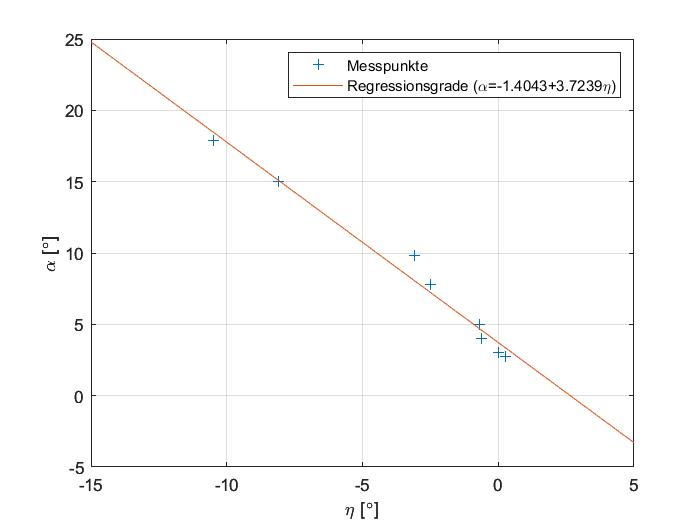
\includegraphics[width=0.7\textwidth]{./Bilder/alpha_eta_plot.jpg}
	\caption{$\alpha$ über $\eta$ der DO-28}
	\label{fig:alpha_eta_DO28}
\end{figure}

\subsection{Auftriebsbeiwert $C_{A}$ über Anstellwinkel $\alpha$}

\begin{figure}[H]
	\centering	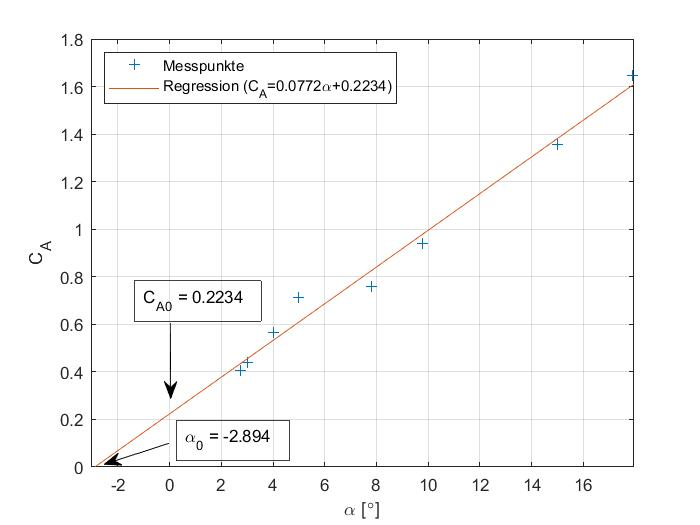
\includegraphics[width=0.7\textwidth]{./Bilder/CA_alpha_plot.jpg}
	\caption{$C_{A}$ über $\alpha$ der DO-28}
	\label{fig:CA_alpha_DO28}
\end{figure}

\subsection{Auftriebsbeiwert $C_{A}$ über Widerstandsbeiwert $C_{W}$}

\begin{figure}[H]
	\centering	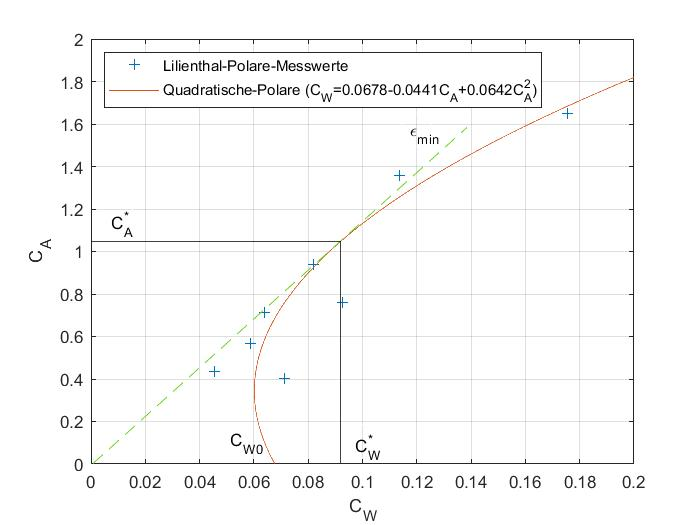
\includegraphics[width=0.7\textwidth]{./Bilder/CA_CW_DO28_NEU.jpg}
	\caption{$C_{A}$ über $C_{W}$ der DO-28}
	\label{fig:CA_CW_DO28}
\end{figure}

\subsection{Widerstand $W$ über Fluggeschwindigkeit $V$}

\begin{figure}[H]
	\centering	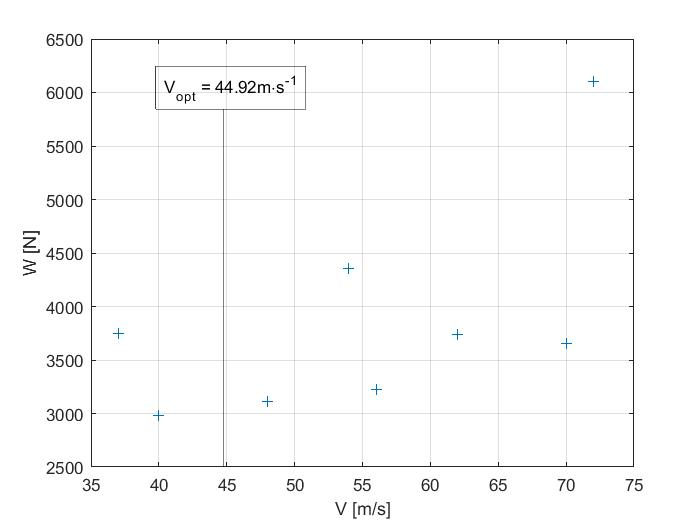
\includegraphics[width=0.7\textwidth]{./Bilder/W_V_DO28_NEU.jpg}
	\caption{$W$ über $V$ der DO-28}
	\label{fig:W_V_DO28}
\end{figure}

Äquivalent zu Abschnitt \ref{ss:W_V} wurde hier $V_{opt}$ und $W_{min}$ mittels der Gleichungen \ref{eq:V_opt} und \ref{eq:W_min} bestimmt. Dabei wurde $G$ und $\rho$ aus den 8 Flugabschnitten gemittelt zu \SI{35728}{\ \newton} und 1,21 \SI{}{\kilogram\ \meter^{-3}}.

\subsection{Fluggeschwindigkeit $V$ und Staudruck $q$ über Anstellwinkel $\alpha$}

\begin{figure}[H]
	\centering	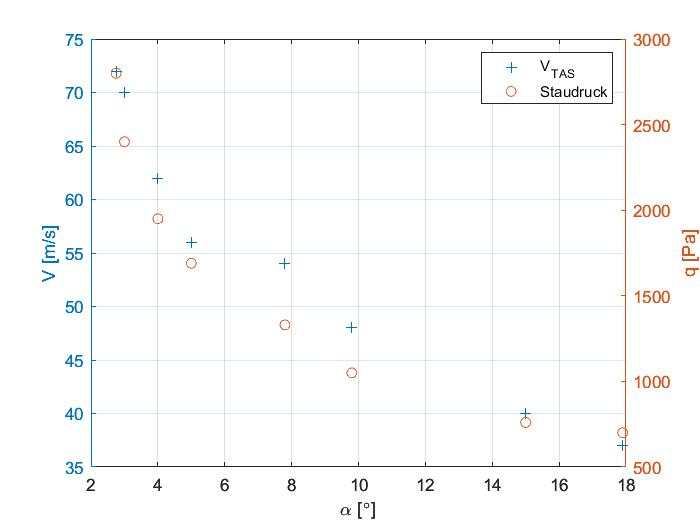
\includegraphics[width=0.7\textwidth]{./Bilder/V_q_alpha.jpg}
	\caption{$V$ und $q$ über $\alpha$ der DO-28}
	\label{fig:V_q_alpha_DO28}
\end{figure}